%%%%%%%%%%%%%%%%%%%%%%%%%%%%%%%%%%%%%%%%%%%%%%%%%%%%%%%%%%%%%%%%%%%%%%%%%%%%%%%%%%%%%%%%%%%%%%%%%%%%%%%%%%%%%%%%%%%%%%%%%%%%%%%%%%%%%%%%%%%%%%%%%%%%%%%%%%%%%%%%%%%%%%%%%%%%%%%%%%%%%%%%%%%%%%%%%%%%%%%%%%%%%%%%%%%%%%%%%%%%%%%%%%%%%%%%%
\iffalse\fi
%%%%%%%%%%%%%%%%%%%%%%%%%%%%%%%%%%%%%%%%%%%%%%%%%%%%%%%%%%%%%%%%%%%%%%%%%%%%%%%%%%%%%%%%%%%%%%%%%%%%%%%%%%%%%%%%%%%%%%%%%%%%%%%%%%%%%%%%%%%%%%%%%%%%%%%%%%%%%%%%%%%%%%%%%%%%%%%%%%%%%%%%%%%%%%%%%%%%%%%%%%%%%%%%%%%%%%%%%%%%%%%%%%%%%%%%%

\documentclass[12pt, letterpaper]{article}

\usepackage{../../../../texmf/mathematics}

\title{\color{BlueGreen}\textbf{Arithmetical Logical Unit Design}}
\author{
\textcolor{OliveGreen}{LazR} \textcolor{Mahogany}{('3')} \\
\textcolor{Lavender}{Alexxia}
                                        }
\date{18th of April, 2025} 

\begin{document}

\maketitle

\newpage

\tableofcontents

\newpage

\Section{1}{Abstract}

This project presents the design and implementation of an \textcolor{cyan}{Arithmetic Logic Unit} (ALU)
capable of performing both logical and arithmetic operations on two 8-bit operands. The ALU supports basic logical operations including
\textcolor{red}{AND}, \textcolor{red}{OR}, and \textcolor{red}{XOR},
as well as fundamental arithmetic operations such as
\textcolor{BurntOrange}{addition}, \textcolor{BurntOrange}{subtraction}, \textcolor{purple}{multiplication}, and \textcolor{purple}{division}.
The goal of this project is to show how these basic operations can be combined into a simple digital system.
The project was developed by \textcolor{Lavender}{Maria - Alexia Crișan} and \textcolor{OliveGreen}{Laz\u{a}r - Iulian Boariu} as part of the \textcolor{cyan}{Calculatoare Numerice} course.

\Section{2}{Finite State Diagram}

\begin{center}
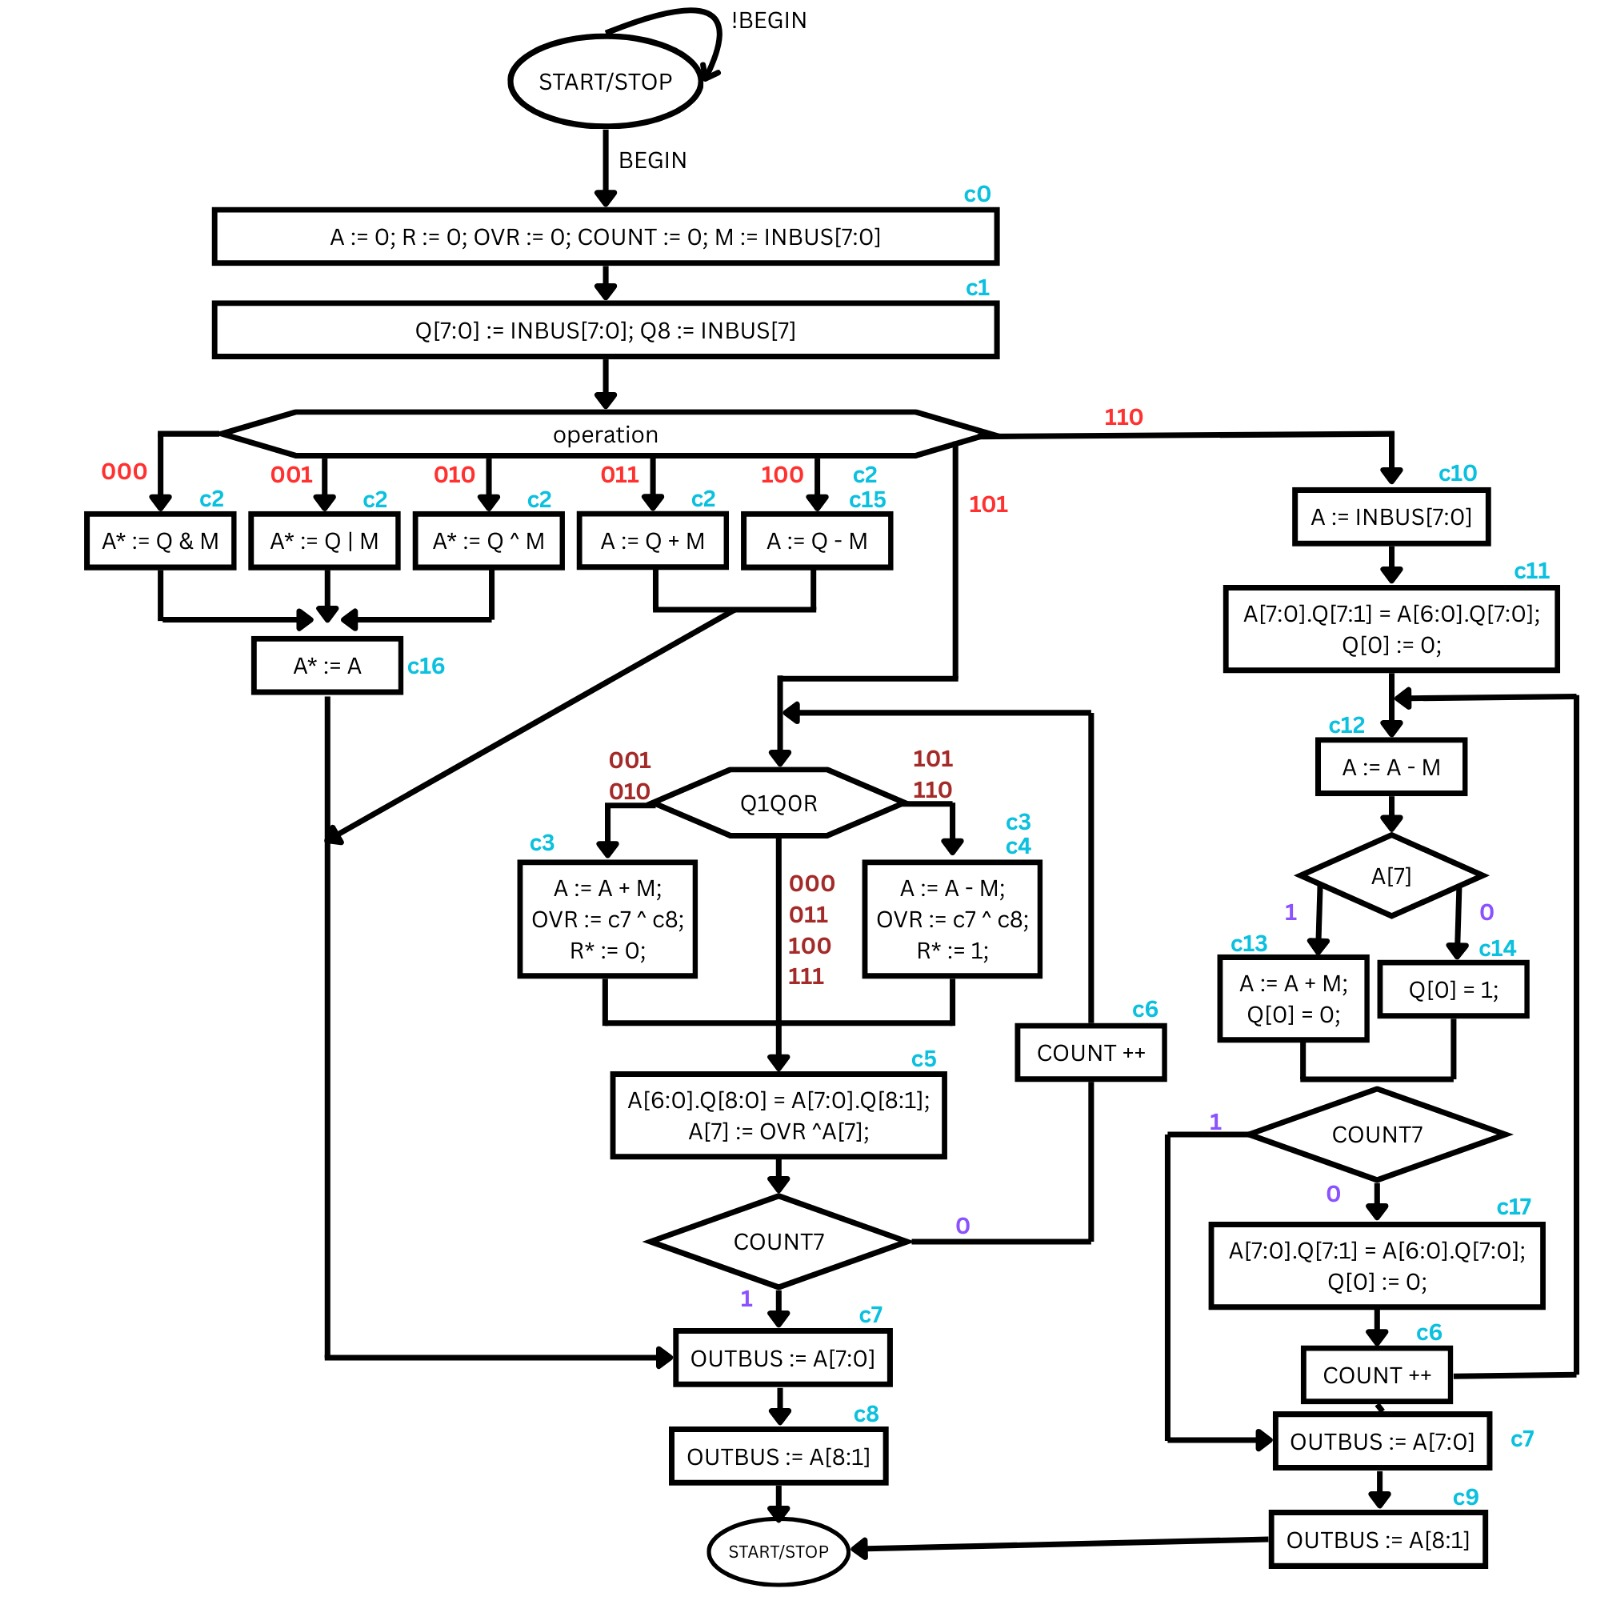
\includegraphics[scale=0.3]{Documentation/FSM}
\end{center}

The diagram illustrates the overall behavior of the ALU, detailing the steps involved in processing data and selecting the appropriate operation based on the provided operation code.\\


The design begins with the initialization of registers and variables, including the two 8-bit operands (Q and M), a remainder register (R), overflow flag (OVR), and a counter.
The control logic then decodes the operation code to determine which operation to execute—logical (AND, OR, XOR) or arithmetic (addition, subtraction, multiplication, division).
Each operation follows a specific path in the flowchart, with conditional branches guiding the transitions between processing stages.\\


Multiplication is implemented using the Modified Booth algorithm, which improves performance by reducing the number of partial products, and is triggered by specific control signals. Similarly, division is handled using the
Restoring Division method, as shown on the right side of the diagram. This method involves conditional subtraction and shifting, iteratively refining the quotient and remainder.\\


The process continues until the counter reaches its limit, after which the final result is written to the output bus. The flowchart provides a structured overview of how the ALU manages complex operations in a controlled and
sequential manner.\\

\Section{3}{Algorithms Used}

\textcolor{RoyalBlue}{\textbf{Modified Booth Multiplication}}

The Modified Booth algorithm is an efficient technique used for signed binary multiplication. It works by encoding the multiplier in groups of three bits, allowing the algorithm to reduce the number of partial products that need to
be generated and added. Instead of performing a simple shift-and-add for every bit of the multiplier, Booth encoding identifies patterns and replaces them with fewer arithmetic operations, such as subtracting or addition. This
method increases speed and reduces the hardware complexity of the multiplier, making it especially useful for larger word sizes or performance-critical designs.\\

\textcolor{CarnationPink}{\textbf{Restoring Division}}

Restoring division is a classic algorithm used for performing binary division by sequentially subtracting the divisor from the partial remainder. At each step, the dividend is shifted left, and the divisor is subtracted from the
current remainder. If the result is positive, the subtraction was valid, and the quotient bit is set to 1. If the result is negative, the original remainder is restored by adding the divisor back, and the quotient bit is set to 0.\\

\Section{4}{ALU Design}

\Section{5}{Control Unit}

The control unit is a key component of the ALU system, responsible for coordinating the execution of operations by generating the necessary control signals at each step. In this project, the control logic is implemented using a
sequence counter, which acts as a simple state machine. Each state corresponds to a specific stage in the execution process, such as loading operands, performing the selected operation, or storing the result. By advancing through
its states in a predefined order, the sequence counter ensures that all operations are carried out in the correct sequence and with proper timing. This approach simplifies the control logic and makes the overall system easier to
manage and debug.\\

To implement the control logic, a \textcolor{YellowGreen}{Modulo-5-sequence} counter was designed, which cycles through five distinct states corresponding to the stages of the ALU operation.
This module serves as the core timing mechanism of the control
unit. The system is composed of several interconnected submodules:
\textcolor{YellowGreen}{Decoder-1-out-of-5}, a \textcolor{YellowGreen}{Modulo-5-counter}, and an \textcolor{YellowGreen}{SR flip-flop}. Each component plays a specific role in generating and controlling the state transitions.\\

1. \textcolor{YellowGreen}{\textbf{Modulo-5-counter}}

This module generates a repetitive sequence of five binary values (from 0 to 4) that represent the current phase. It increments its output on each clock cycle, looping back to zero after reaching four. The modulo-5 behavior
ensures that the control unit progresses through exactly five phases before restarting the sequence.\\

2. \textcolor{YellowGreen}{\textbf{Decoder-1-out-of-5}}

The decoder takes the 3-bit output from the modulo-five counter and activates exactly one of its five outputs at a time. This ensures that only one phase signal is active during each step, allowing precise control over which
control lines are enabled. Essentially, it translates the binary count into a one-hot encoding format, which is easier to use for controlling sequential logic.\\

3. \textcolor{YellowGreen}{\textbf{SR Flip-Flop}}

The Start/Stop latch controls whether the sequence counter is active or halted. It enables or disables the advancement through the counting sequence based on external conditions or control inputs. When the latch is set, the
modulo-5 counter is allowed to advance on each clock cycle, progressing through the defined control states. When reset, the counter is held in place, effectively pausing the control unit. This mechanism provides a simple and
effective way to synchronize the ALU's operation with the system's global control logic.

\begin{center}
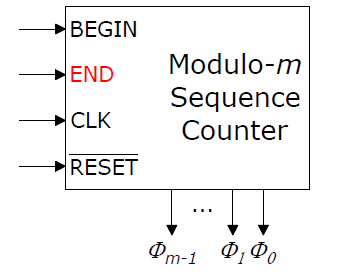
\includegraphics[scale=0.3]{Documentation/modulo_counter}
\end{center}

The picture illustrates the internal structure and signal connections within the \textcolor{YellowGreen}{Modulo-5-sequence} counter used in the control unit.
It shows how the \textcolor{YellowGreen}{Modulo-5-counter}, \textcolor{YellowGreen}{1-out-of-5 Decoder} and the \textcolor{YellowGreen}{Start/Stop} latch are connected to
manage state transitions. 


\begin{center}
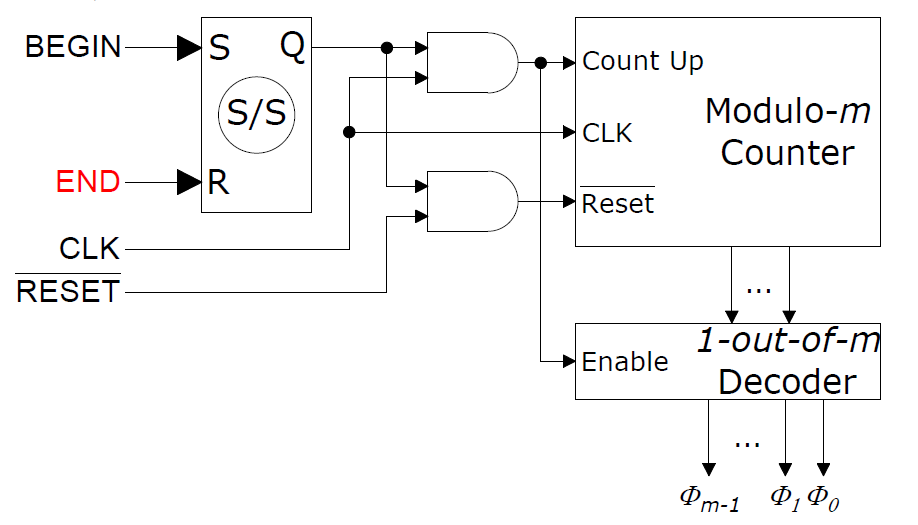
\includegraphics[scale=0.3]{Documentation/sr}
\end{center}

Each operation supported by the ALU has a specific set of control signals that are activated during certain steps of the control sequence. These signals coordinate actions such as loading operands, enabling the ALU,
performing addition or subtraction, and storing the result. The list below outlines the control signals associated with each operation and indicates during which phase (based on the output of the Modulo-5 sequence counter) each
signal is active:\\

\textcolor{ForestGreen}{\textbf{Control Signals by Operation}}\\

1. \textcolor{red}{AND} / \textcolor{red}{OR} / \textcolor{red}{XOR} (Logical Operations)\\

Operation codes: \textcolor{red}{AND}(\textcolor{ForestGreen}{000}), \textcolor{red}{AND}(\textcolor{ForestGreen}{001}), \textcolor{red}{XOR}(\textcolor{ForestGreen}{010})\\

Cycle 0: 

\begin{itemize}
  \item Phase 0: \textcolor{cyan}{c0} -> Load operand M
  \item Phase 1: \textcolor{cyan}{c1} -> Load operand Q
  \item Phase 2: \textcolor{cyan}{c2} -> Enable logic unit
  \item Phase 3: \textcolor{cyan}{c16} -> Store result in A-star based of off op
\end{itemize}


Cycle 9:

\begin{itemize}
  \item Phase 0: \textcolor{cyan}{c7} -> Load result A
  \item Phase 1: \textcolor{cyan}{c8} -> Load result Q
\end{itemize}
---------> Activate \textcolor{red}{END} signal\\

2. \textcolor{BurntOrange}{ADD} / \textcolor{BurntOrange}{SUB} (Arithmetic Operations)\\

Operation codes: \textcolor{BurntOrange}{ADD}(\textcolor{ForestGreen}{011}), \textcolor{BurntOrange}{SUB}(\textcolor{ForestGreen}{100})\\

Cycle 0:

\begin{itemize}
  \item Phase 0: \textcolor{cyan}{c0} -> Load operand M
  \item Phase 1: \textcolor{cyan}{c1} -> Load operand Q
  \item Phase 2: \textcolor{cyan}{c2} -> Triggers addition, the result is stored in A
  \item Phase 2: \textcolor{cyan}{c15} -> Triggers subtraction, the result is stored in A
\end{itemize}


Cycle 9:

\begin{itemize}
  \item Phase 0: \textcolor{cyan}{c7} -> Load result A
  \item Phase 1: \textcolor{cyan}{c8} -> Load result Q
\end{itemize}
---------> Activate \textcolor{red}{END} signal\\

3. \textcolor{purple}{MULTIPLICATION} (Modified Booth)\\

Operation codes: \textcolor{purple}{MULTIPLICATION}(\textcolor{ForestGreen}{101})\\

Cycle 0:

\begin{itemize} \item Phase 0: \textcolor{cyan}{c0} -> Load operand M and initialize A, COUNT, R, OVR \item Phase 1: \textcolor{cyan}{c1} -> Load operand Q and Q8 \end{itemize}

Cycle 1 - 8:

\begin{itemize} \item Phase 0: \textcolor{cyan}{c3} -> Triggers addition for Q1Q0R in {001, 010, 101, 110}, R* = 0, OVR is calculated \item Phase 0: \textcolor{cyan}{c4} -> Additional signal for subtraction for Q1Q0R in {101, 110}, R* = 1, OVR is calculated \item Phase 1: \textcolor{cyan}{c5} -> Triggers right shift \item Phase 2: \textcolor{cyan}{c6} -> COUNT is updated \end{itemize}

Cycle 9:

\begin{itemize} \item Phase 0: \textcolor{cyan}{c7} -> Load result A \item Phase 0: \textcolor{cyan}{c5} -> Triggers final right shift \item Phase 1: \textcolor{cyan}{c8} -> Load result Q \end{itemize} ---------> Activate \textcolor{red}{END} signal\\

4. \textcolor{purple}{DIVISION} (Restoring Division)\\

Operation codes: \textcolor{purple}{DIVISION}(\textcolor{ForestGreen}{110})\\

Cycle 0:

\begin{itemize} \item Phase 0: \textcolor{cyan}{c0} -> Load operand M \item Phase 1: \textcolor{cyan}{c1} -> Load operand Q \item Phase 2: \textcolor{cyan}{c10} -> Load operand A (first half of the dividend) \item Phase 3: \textcolor{cyan}{c11} -> Triggers initial left shift \end{itemize}

Cycle 1 - 8:

\begin{itemize} \item Phase 0: \textcolor{cyan}{c12} -> Triggers subtraction \item Phase 1: \textcolor{cyan}{c13} -> Triggers addition when A[7] = 1, updates Q[0] = 0 \item Phase 1: \textcolor{cyan}{c14} -> Updates Q[0] = 1 \item Phase 2: \textcolor{cyan}{c6} -> COUNT is updated \item Phase 3: \textcolor{cyan}{c17} -> Triggers left shift \end{itemize}

Cycle 9:

\begin{itemize} \item Phase 0: \textcolor{cyan}{c7} -> Load result A \item Phase 0: \textcolor{cyan}{c9} -> Load result Q \end{itemize} ---------> Activate \textcolor{red}{END} signal\


\end{document}
